\chapter{Lösungen}

Es gibt verschiedene Lösungen für den \IM. Zunächst möchte ich eine vorstellen, die dem eigentlichen \IM aus dem Weg geht und einen anderen Ansatz verfolgt: Das Ersetzen der relationalen Datenbank mit einem anderen Datenbankmanagmentsystem. Danach beschäftige ich mich mit dem \term{Object-Relational Mapping}%erstes Vorkommen
, welches die klassische Lösung des \IM ist.

\section{Ersetzen der Datenbank}

Zunächst werden \term{Objektdatenbankmanagementsysteme} (OODBMS bzw ODBMS) betrachtet. %erstes Vorkommen
\begin{definition}[ODBMS]
An object-oriented database system must satisfy two criteria: it should be a DBMS, and it should be an object-oriented system, i.e., to the extent possible, it should be consistent with the current crop of object-oriented programming languages. The first criterion translates into five features: persistence, secondary storage management, concurrency, recovery and an ad hoc query facility. The second one translates into eight features: complex objects, object identity, encapsulation, types or classes, inheritance, overriding combined with late binding, extensibility and computational completeness. \cite{odbms-manifesto}
\end{definition}
\noindent Der \IM wird überbrückt, indem das \RDBMS mit einem System ersetzt wird, welches den Prinzipien des objektorientierten Paradigma folgt. Das bedeutet, dass viele Ausprägungen der Probleme die vorher genannt wurden auf natürliche Weise nicht mehr gelöst werden müssen. Gerade die Eigenschaften des zweiten Kriteriums wie: \term{object identity}, \term{encapsulation} und \term{inheritance} lösen die schwierigsten Probleme die in \cite[S. 38]{classification} beschrieben werden. Das Objekt welches persistent gemacht werden soll, muss nicht mehr in atomare, in einer Datenbank speicherbare Datentypen zerlegt werden und beim Laden wieder zusammengesetzt werden. Gerade für komplexe Objekte mit vielen Abhängigkeiten untereinander ist dies ein enormer Vorteil. Der Grund warum dies mit \ODBMSs so gut funktioniert ist, dass diese Systeme nicht mehr Relationen als Basis benutzen, sondern man sich veranschaulicht vorstellen kann, dass das Objekt „so wie es ist“ in der Datenbank gespeichert wird.\\
Man könnte also annehmen, dass \ODBMSs die sinnvollste, einfachste und ökonomischsten Lösungen für den \IM sind. De facto ist es aber so, dass \ODBMSs sich noch nicht so durchsetzen konnten, wie man anfänglich erwartet hatte. Wenn ein \ODBMS keine Relationen mehr benutzt, dann ist auch klar, dass man die Vorteile, die ein relationales \DBMS mit sich bringt, verliert. In \cite{what-ever-happened-to-odbmss} werden weitere folgende Gründe genannt, warum \ODBMS nicht so erfolgreich wurden:
\begin{itemize}
\item \RDBMSs wurden mit objektorientierten Features bestückt und entwickelten sich so weiter. Dadurch gewannen die bereits in der Indstrie etablierten Datenbanksysteme wieder ihre verlorene Popularität gegenüber \ODBMSs zurück.
\item In \ODBMS ist es performanter komplexe Mengen von Datenobjekten zu speichern, \ODBMS können den Speicher des Clients direkt als Cache verwalten und der Optimierer des Systems wählt die beste Form für das physikalische Design der Datenbank. Diesen Vorteil reduzierten die \RDBMSs indem sie ihre Prozesse Daten aus Tabellen abzufragen, weiter optimierten.
\item Zwar ist es vorteilhafter eine komplexes, objektorientiertes Schema einer Applikation mit einem \ODBMS persistent zu machen, doch die Bereiche in denen diese Schemas existieren und \ODBMSs ihre Anwendungen finden sind nur kleine Nischenmärkte.
\item \RDBMSs stützen sich auf den lang etablierten Standard SQL. Die Object Database Management Group entwickelt zwar Standards für \ODBMSs und \ORM-Produkte, aber der Standard ist nicht weit verbreitet und zu wenige Hersteller unterstützen den Standard, um ihn wirklich für die Industrie relevant zu machen. So konnte sich zum Beispiel der OQL-Standard (\term{Object Query Language}) nie richtig durchsetzen.
\item Das Fehlen von SQL wurde zu spät von Herstellern als gravierender Nachteil der \ODBMSs realisiert.
\item Firmen die bereits ein bestehendes \RDBMS, bzw die Abwandlung davon als \ORDBMS als bevorzuge Datenbanklösung benutzen, wechseln gerechtfertigter Weise zu keiner neuen Lösung. Nur wenn die neuen Systeme einen unwiderstehlich lukrativen, wirtschaftlichen Vorteil gegenüber den alten bieten würden - was \ODBMS nicht können - gäbe es eine Chance, \RDBMSs in ihrer Vormachtsstellung in Gefahr zu bringen. Hinzu kommt, dass bestehende Hersteller von \RDBMSs mehr Ressourcen und Mittel z.~B. fürs Marketing zur Verfügung haben, weil sie bereits eine größere Basis an verkauften Produkten besitzen.
\end{itemize}
Die genannte Erweiterung der relationalen Datenbankmanagmentsysteme mit objektorientierten Features bezeichnet man als %erstes Vorkommen
\term{Objektrelationales Datenbankmanagementsystem} kurz \ORDBMS. Die Definition eines \ORDBMS ist schwer zu formulieren. Um genauer zu sein, gibt es überhaupt keinen Standard oder eine von allen anerkannte wissenschaftliche Arbeit, die einem erlauben würde ein \ORDBMS zu charakterisieren. \\
Der Übergang von einem \RDBMS zu einem \ORDBMS kann also mehr oder weniger fließend sein. Somit können relationale Systeme schon als objektrelationale Systeme bezeichnet werden, wenn sie nur ein objektorientiertes Feature umsetzen. In \cite{ordbms-the-road-ahead} wird versucht die Charakteristika eines \ORDBMS so zu beschreiben: 
\begin{itemize}
\item Erweiterung von Basisdatentypen
\item Unterstützung von komplexen Objekten
\item Vererbung
\end{itemize}
Es ist also nicht leicht ein konkretes \DBMS als \ORDBMS oder \RDBMS zu bezeichnen \cite{ordbms-the-next-wave}. Um trotzdem ein Gefühl entwickeln zu können, wie weit sich die Hersteller um die Entwicklung ihres \RDBMS zu einem \ORDBMS kümmern, zeigt Abbildung \ref{object-relational-dbms} eine mögliche Klassifizierung einiger bekannter Datenbankmanagmentsysteme (Quelle für die Auswahl der Datenbanksysteme: Evans Data Corp: Users’ Choice Database Servers (2008)). Desto weiter ein Datenbanksystem auf dem Strahl weiter links steht, desto eher ist es meiner Einschätzung nach als reines \OODBMS charakterisierbar. Desto weiter ein \DBMS rechts auf dem Strahl erscheint, desto weniger objektrelationale Features unterstützt es. Es ist zu beachten, dass die meisten \RDBMS sich in Richtung einer Position weiter links auf dem Strahl entwickeln, während sich nur wenige \OODBMS in die relationale Richtung bewegen.
\begin{figure}[htbp]
  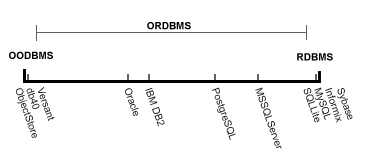
\includegraphics[width=\textwidth]{figures/ordbms}
  \caption{Klassifizierung beliebter Datenbankmanagmentsysteme}
  \label{object-relational-dbms}
\end{figure}
Anbei noch ein paar Anmerkungen zur Platzierung der verschiedenen \DBMS auf dem Strahl:
\paragraph{Oracle11}
Mit \term{Oracle Objects} können benutzerdefinierte Objekte (Objekttypen) in der Datenbank gespeichert werden. Diese Objekte werden aus Basisdatentypen oder anderen Objekten zusammengesetzt. Zusätzlich zu der Definition des Objekttypen können auch Methoden definiert werden. Danach ist es möglich diesen Typen in einer Tabelle zu verwenden. Dabei kann dieser Objekttyp mit verschiedenen anderen relationalen Informationen vermischt werden. Wird der Objekttyp als Typ einer Tabelle benutzt (\term{Object Tables}) kann sowohl auf das ganze Objekt (und dessen definierten Methoden), als auch auf jede Spalte einzeln zugegriffen werden. D.~h. es ist möglich, das Objekt als Objekt oder auch als eine einzelne Zeile mit Spalten anzusprechen, um relationale Features nutzen zu können. Es sind Referenzen auf Objekte in Tabellen möglich, es gibt Collections und Typen können voneinander abgeleitet werden. Extensions für die Spracherweiterung gibt es für C++, .NET und Java und natürlich über das eigene \term{Call Level Interface}; Zusätzlich gibt es eine SQL Spracherweiterung (inklusive DDL Statements) \cite{oracle-db-object-relational-guide}.\\
Diese Sammlung von Eigenschaften und Fähigkeiten macht Oracle für mich zu dem DBMS welches man am ehesten als \ORDBMS bezeichnen kann.\\

\paragraph{DB2}
In DB2 ist es ebenfalls möglich benutzerdefinierte Typen zu erstellen. Diese \term{distinct Types} können von Basisdatentypen abgeleitet werden und sind somit auch gut in den Database-Manager integriert. Zusätzlich können diesen Typen auch benutzerdefinierte Funktionen zugewiesen werden. Es wird ein Grundstock von Multimedia Datentypen mitgeliefert: Audio, Bilder, Video und Text. Von Funktionen können Tabelle statt Skalare zurückgegeben werden. Somit ist es möglich, jede Datenquelle als Tabelle darzustellen und so die gewohnten relationalen Features zu benutzen. Mit dem \term{structured Type} ist auch Vererbung möglich, denn \term{structured Types} können von anderen Typen abgeleitet werden. Dadurch können dann Tabellen von einem \term{structured Type} ebenso wie in Oracle als Objekttabellen erstellt werden und diese wiederum von anderen Tabellen deren Spalten und Methoden erben. Auch hier ist es möglich die Objekte in der Tabelle als separate Spalten anzusprechen. Zusätzlich werden \term{Path-Expressions} für die Abfrage von Beziehungen von Objekten genutzt und \term{Object Views} können erstellt werden. \cite{db2-object-relational-highlight}.\\

\paragraph{PostgreSQL}
PostgreSQL tendiert in die \ODBMS-Richtung, da es auch die Vererbung in Tabellen unterstützt. Bei einem \term{CREATE TABLE} kann die Option \term{INHERITS} mit angegeben werden. Die Attribute der Elterntabelle werden dann auf die Kindtabellen übertragen. Zusätzlich versucht PostgreSQL den SQL3 Standard (in Entwicklung) umzusetzen. Deshalb ermöglicht es jetzt schon z.~B. in Funktionen Tabellen zurückzugeben, oder die Verwaltung von XML als Datentypen. Es erweitert auch einige seiner Basisdatentypen zu Multimediatypen. \\

\paragraph{Microsoft SQL Server}
Features die man bei IBM und Oracle findet, findet man weniger in den Feature-Listen von Microsoft SQL Server (\cite{sql-server-2008}). Ich denke, das liegt daran, dass Microsoft andere Wege gefunden hat mit dem \IM umzugehen \cite{meijer-linq-visual-basic}. So findet sich z.~B. LINQ als objektrelationales Feature wieder. Trotzdem liefert auch Microsoft eine Möglichkeit für Multimedia Datentypen (\term{Large User-Defined Types: UDTs}). Zu diesen Typen werden auch neue Definitionen von Aggregatfunktionen angeboten: \term{Large User-Defined Aggregates: UDAs}. Mit \term{ORDPATH} können Hierarische Daten als Baum abgespeichert werden.\\

\paragraph{Caché von Intersystems (nicht abgebildet)} Caché von Intersystems \cite{cache-intersystems} bezeichnet sich selbst als postrelationales Datenbanksystem. In der Abbildung taucht der Name nicht auf, da man es an jedem Punkt des Strahls zeichnen könnte. Caché bietet sowohl eine relationale als auch eine objektorientierte Datenbankansicht. Die Datenbasis ist weder relational noch objektorientiert, sondern hierarchisch.\\

\section{Object-relational Mapper}

Zwar lösen \OODBMSs die Schwierigkeiten die der \IM mit sich bringt, doch je nachdem welches \ORDBMS oder \RDBMS benutzt wird, gibt es noch genug Probleme die auf Softwareebene gelöst werden müssen. Es lässt sich nur schwer vorraussagen, wann sich Datenbanksysteme so verändern, dass es in der praktischen Anwendung überhaupt keine reinen relationalen Datenbanken mehr gibt. Deshalb gibt es genug Szenarien in denen der \IM, oder Teile des \IM nach wie vor eine große Rolle spielen und eine universellere Methode zur Lösung gefunden werden muss.\\
\\
Wenn man die zu lösenden Schwierigkeiten betrachtet, fällt auf, dass die meisten dadurch entstehen, dass ein Element aus dem objektorientierten Paradigma im relationalen Schema nicht abgebildet werden kann. Es muss also ein Element (oder eine Kombination aus mehreren) des relationalen Models gefunden werden, das dieses Element des objektorientierten Models modellieren kann. Die Abbildungen zwischen diesen Elementen - auch \term{Mapping} genannt - können in verschiedenen Weisen realisiert werden. Eine Lösung des \IM, die eine Menge von \term{Mappings} definiert und relationale Elemente in objektorientierte Elemente oder vice versa überführt, nennt man einen \term{Object Relational Mapper} %erstes Vorkommen
oder kurz: \ORM. \\
Im folgenden Kapitel konzentriere ich mich auf \term{Object-relational Mappings}. Ich stelle verschiedene schon erforschte \term{Mappings} für bestimmte Kernprobleme vor und erkläre die Probleme, die dabei entstehen. \\
Im Kapitel darauf betrachte ich ein paar Implementierungen dieser Strategien und zeige Vor- und Nachteile bei der Lösung dieser Probleme.\\
